% Evidence gap map — bias x mitigation intersections
% Compile: pdflatex evidence_gap.tex
% Data source: evidence_gap_map_data.json (78 studies, Jan 2017 – Mar 2026)
\documentclass[tikz, border=15pt]{standalone}
\usepackage[T1]{fontenc}
\usepackage{lmodern}
\usepackage{amssymb}
\usepackage{xcolor}
\usepackage{tikz}
\usetikzlibrary{positioning,shapes.geometric,calc,fit,backgrounds}

%------- Colours -------
\definecolor{binZero}{HTML}{FFFFFF}
\definecolor{binLow} {HTML}{FCEC94}
\definecolor{binMid} {HTML}{FCC573}
\definecolor{binHigh}{HTML}{FD7D22}
\definecolor{binTop} {HTML}{B71C24}

\definecolor{grpPre} {HTML}{1F78B4}
\definecolor{grpFeat}{HTML}{2CA25F}
\definecolor{grpProt}{HTML}{6A3D9A}
\definecolor{grpCol} {HTML}{E66101}
\definecolor{grpDom} {HTML}{8C2D04}
\definecolor{grpFdn} {HTML}{377EB8}
\definecolor{grpPost}{HTML}{E31A1C}

\definecolor{biasA}{HTML}{1F4E9D}
\definecolor{biasB}{HTML}{2E8B57}
\definecolor{biasC}{HTML}{6A3D9A}
\definecolor{biasD}{HTML}{E07B00}
\definecolor{biasE}{HTML}{C1272D}
\definecolor{biasF}{HTML}{8A6D1F}
\definecolor{biasG}{HTML}{C2185B}
\definecolor{biasH}{HTML}{00838F}

\definecolor{barBlue} {HTML}{3A74B8}
\definecolor{gridGrey}{HTML}{BFBFBF}

%------- Helpers -------
\newcommand{\biasnum}[2]{%
  \tikz[baseline=-0.6ex]\node[circle,fill=#1,text=white,inner sep=0pt,
    minimum size=4.6mm,font=\bfseries\small]{#2};}

\makeatletter
\newcommand{\pickbin}[1]{%
  \ifnum#1=0  \def\binColor{binZero}\else
  \ifnum#1<3  \def\binColor{binLow} \else
  \ifnum#1<6  \def\binColor{binMid} \else
  \ifnum#1<12 \def\binColor{binHigh}\else
              \def\binColor{binTop} \fi\fi\fi\fi}
\makeatother

\newcommand{\gStrong}{$\bigstar$}
\newcommand{\gMod}   {$\blacktriangle$}
\newcommand{\gMixed} {$\bullet$}
\newcommand{\gNone}  {\textendash}

\newcommand{\RH}{1.1}

\newcommand{\cell}[4]{%
  \pickbin{#3}%
  \begin{scope}
    \fill[\binColor] (#1,#2) rectangle ++(1,\RH);
    \draw[gridGrey,line width=0.35pt] (#1,#2) rectangle ++(1,\RH);
    \ifnum#3>10
      \node[font=\bfseries\large,white] at (#1+0.5,{#2+\RH*0.65}) {#3};
    \else\ifnum#3>5
      \node[font=\bfseries\large,black] at (#1+0.5,{#2+\RH*0.65}) {#3};
    \else
      \node[font=\normalsize,black]     at (#1+0.5,{#2+\RH*0.65}) {#3};
    \fi\fi
    \def\glyph{}%
    \ifnum\pdfstrcmp{#4}{strong}=0 \def\glyph{\gStrong}\fi
    \ifnum\pdfstrcmp{#4}{mod}   =0 \def\glyph{\gMod}   \fi
    \ifnum\pdfstrcmp{#4}{mixed} =0 \def\glyph{\gMixed} \fi
    \ifnum\pdfstrcmp{#4}{none}  =0 \def\glyph{\gNone}  \fi
    \node[font=\normalsize] at (#1+0.5,{#2+\RH*0.25}) {\glyph};
  \end{scope}}

\begin{document}
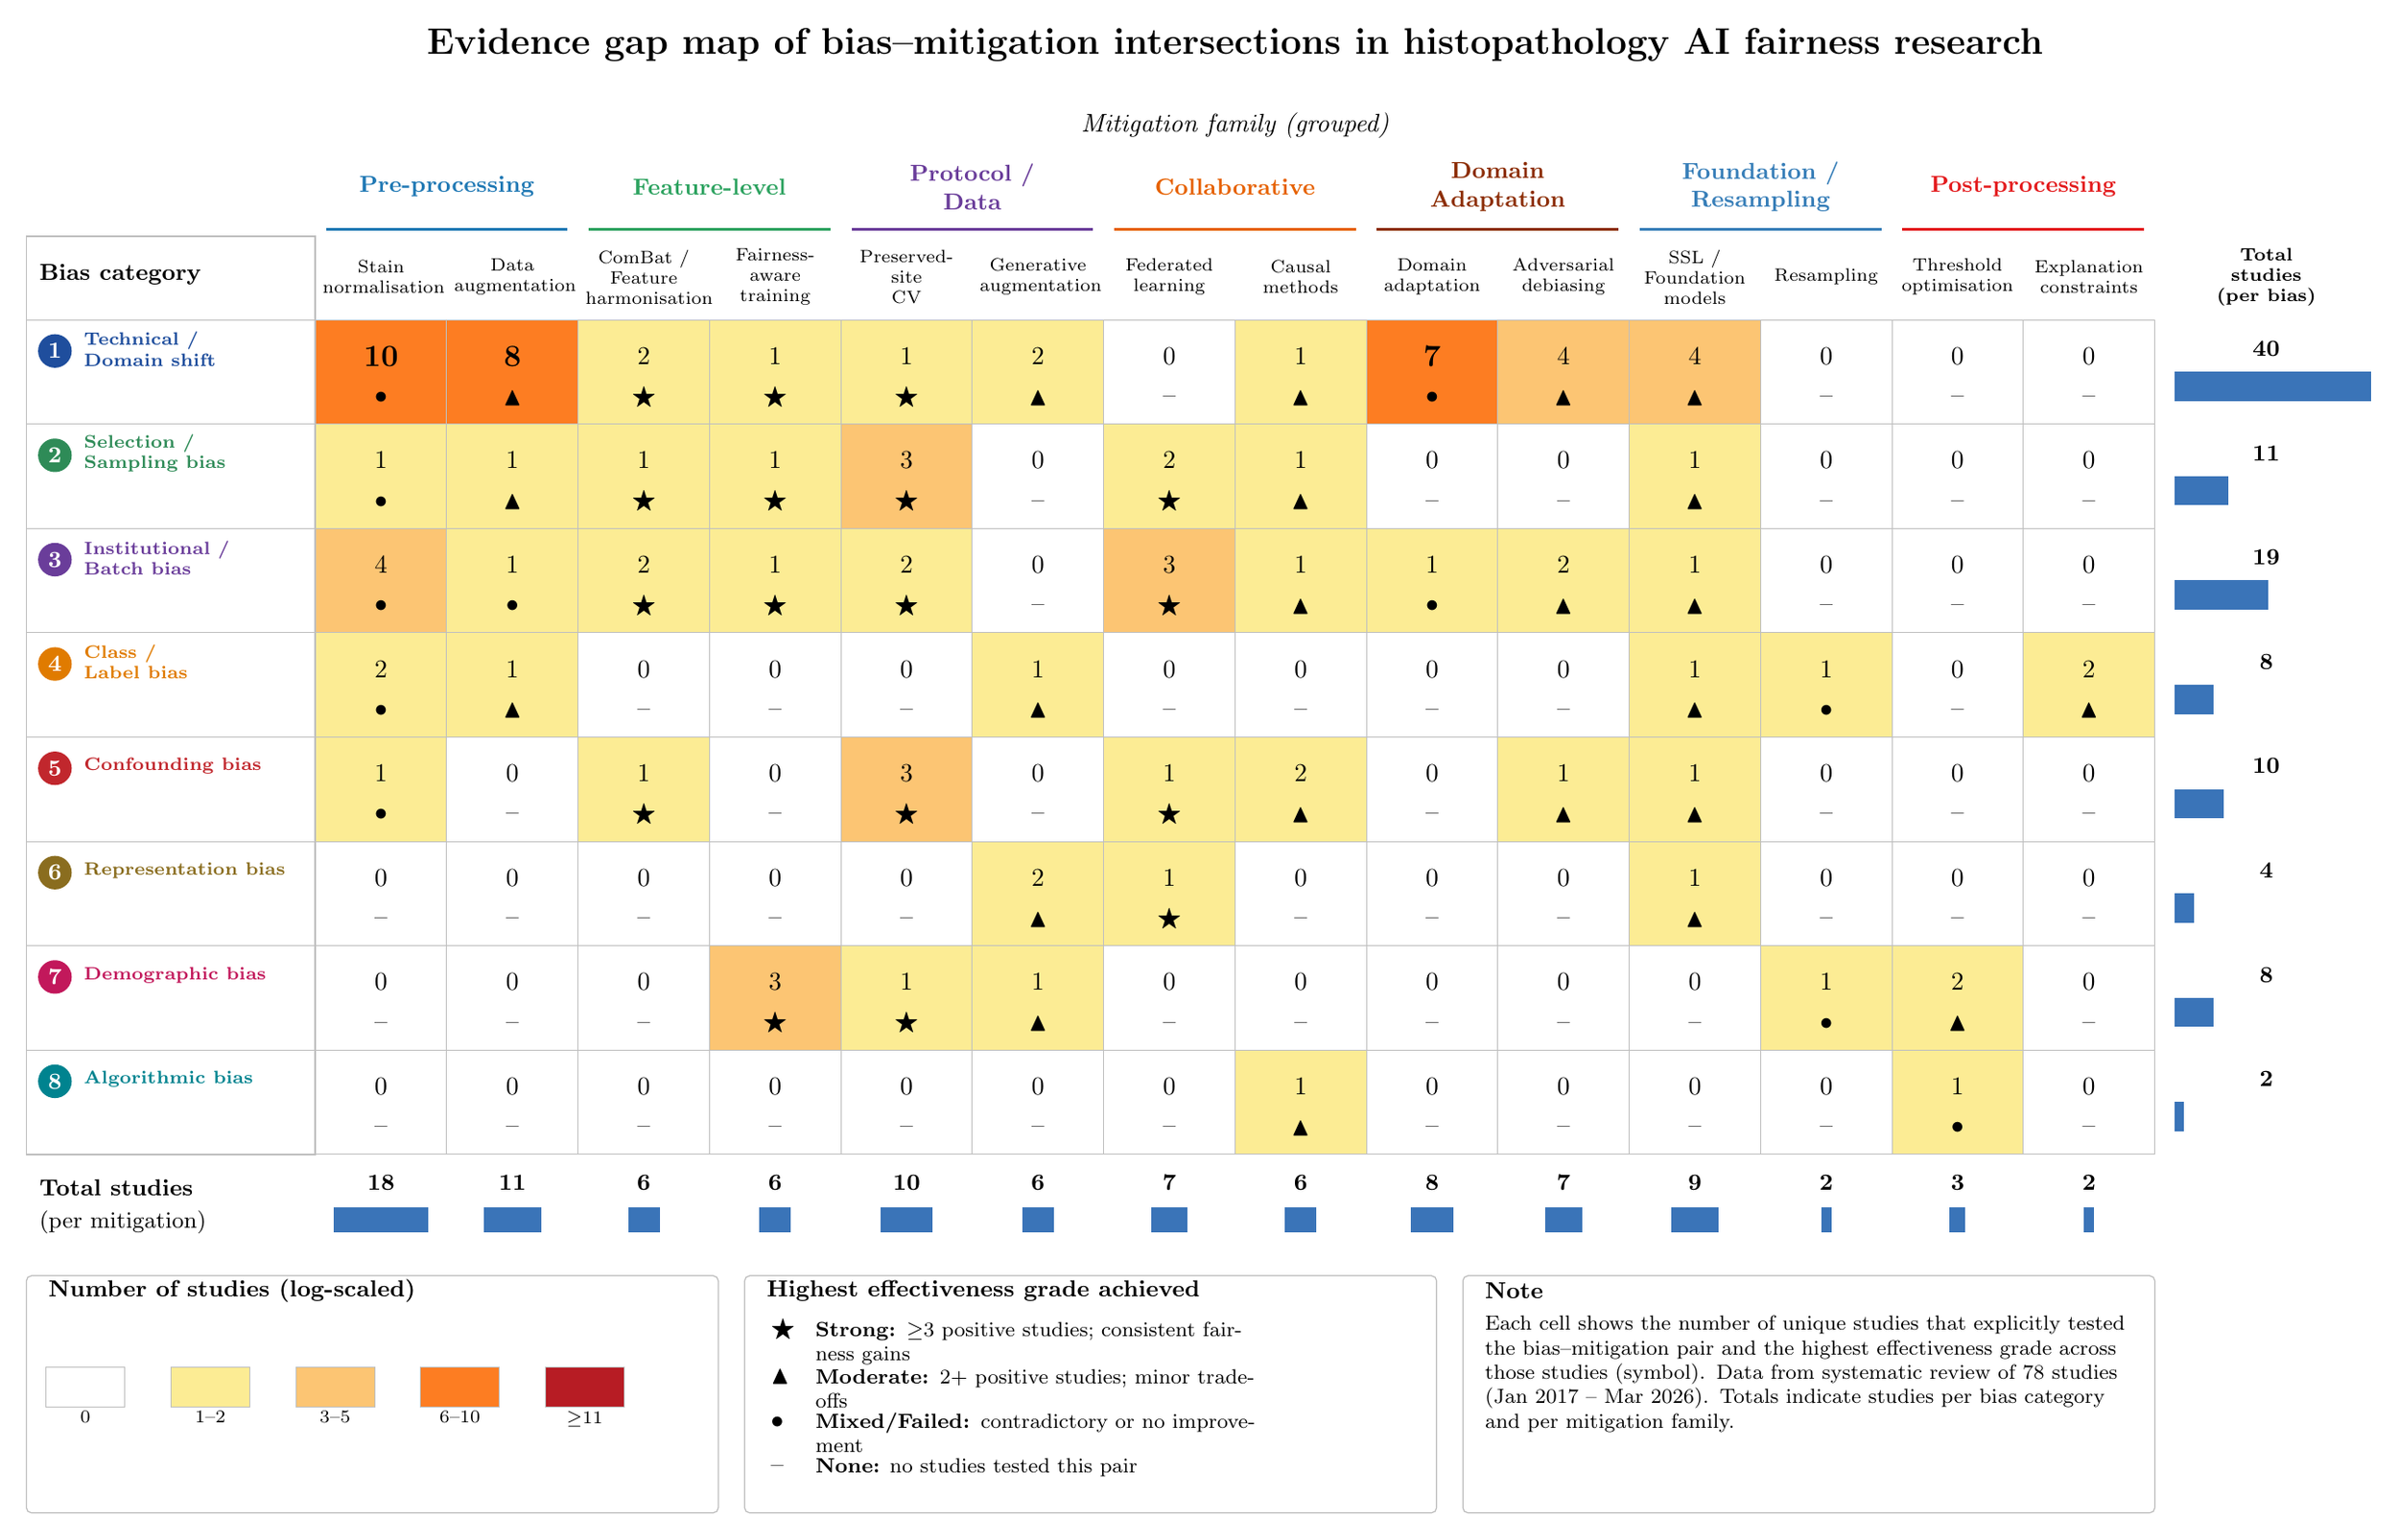
\begin{tikzpicture}[x=1.80cm, y=1.30cm,
    every node/.style={inner sep=1pt,outer sep=0pt}]

\def\BLEFT{-2.20}
\def\YTOP{9.9}
\def\YBOT{1.1}
\def\YHDRTOP{10.78}

% ========== TITLE ==========
\node[font=\bfseries\Large] at (7.0,12.8)
  {Evidence gap map of bias--mitigation intersections in histopathology AI fairness research};

% ========== MITIGATION FAMILY header ==========
\node[font=\itshape] at (7.0,11.95) {Mitigation family (grouped)};

\foreach \xa/\xb/\txt/\col in {%
  0/2/{Pre-processing}/grpPre,
  2/4/{Feature-level}/grpFeat,
  4/6/{Protocol /\\Data}/grpProt,
  6/8/{Collaborative}/grpCol,
  8/10/{Domain\\Adaptation}/grpDom,
  10/12/{Foundation /\\Resampling}/grpFdn,
  12/14/{Post-processing}/grpPost}{
  \node[font=\bfseries\small,\col,align=center,text width=2.80cm]
       at ({(\xa+\xb)/2},11.30) {\txt};
  \draw[\col,line width=1pt] (\xa+0.08,10.85) -- (\xb-0.08,10.85);
}

% ========== COLUMN HEADERS ==========
\foreach \i/\txt in {%
  0/{Stain\\normalisation},
  1/{Data\\augmentation},
  2/{ComBat /\\Feature\\harmonisation},
  3/{Fairness-aware\\training},
  4/{Preserved-site\\CV},
  5/{Generative\\augmentation},
  6/{Federated\\learning},
  7/{Causal\\methods},
  8/{Domain\\adaptation},
  9/{Adversarial\\debiasing},
  10/{SSL /\\Foundation\\models},
  11/{Resampling},
  12/{Threshold\\optimisation},
  13/{Explanation\\constraints}}{
  \node[font=\scriptsize,align=center,text width=1.60cm]
       at (\i+0.5,10.35) {\txt};
}

\node[font=\scriptsize\bfseries,align=center,text width=1.5cm]
     at (14.85,10.35) {Total studies\\(per bias)};

% ========== BIAS CATEGORY COLUMN BOX ==========
\draw[gridGrey, line width=0.55pt]
  (\BLEFT, \YBOT) rectangle (0, \YHDRTOP);
\draw[gridGrey, line width=0.35pt]
  (\BLEFT, \YTOP) -- (0, \YTOP);
\node[font=\bfseries\small, anchor=west] at (\BLEFT+0.08, 10.38)
  {Bias category};

% ========== ROW LABELS ==========
\newcommand{\rowlabel}[5]{%
  \pgfmathsetmacro{\yc}{9.9 - 1.1*(#1) + 0.55}%
  \ifnum#1<8
    \draw[gridGrey,line width=0.25pt]
      (\BLEFT,{9.9-1.1*(#1)}) -- (0,{9.9-1.1*(#1)});
  \fi
  \node[anchor=west] at (\BLEFT+0.07, \yc+0.22) {\biasnum{#2}{#3}};
  \node[font=\bfseries\scriptsize,#2,anchor=west,align=left,text width=3.10cm]
       at (\BLEFT+0.42, \yc+0.24) {#4};
  \node[font=\scriptsize,anchor=west,align=left,text width=2.50cm]
       at (\BLEFT+0.08, \yc-0.30) {#5};
}

\rowlabel{1}{biasA}{1}{Technical /\\Domain shift}{}
\rowlabel{2}{biasB}{2}{Selection /\\Sampling bias}{}
\rowlabel{3}{biasC}{3}{Institutional /\\Batch bias}{}
\rowlabel{4}{biasD}{4}{Class /\\Label bias}{}
\rowlabel{5}{biasE}{5}{Confounding bias}{}
\rowlabel{6}{biasF}{6}{Representation bias}{}
\rowlabel{7}{biasG}{7}{Demographic bias}{}
\rowlabel{8}{biasH}{8}{Algorithmic bias}{}

% ========== DATA CELLS ==========
% Row 1 (y=8.8) Technical / Domain shift
\cell{0}{8.8}{10}{mixed}\cell{1}{8.8}{8}{mod}\cell{2}{8.8}{2}{strong}\cell{3}{8.8}{1}{strong}
\cell{4}{8.8}{1}{strong}\cell{5}{8.8}{2}{mod}\cell{6}{8.8}{0}{none}\cell{7}{8.8}{1}{mod}
\cell{8}{8.8}{7}{mixed}\cell{9}{8.8}{4}{mod}\cell{10}{8.8}{4}{mod}\cell{11}{8.8}{0}{none}
\cell{12}{8.8}{0}{none}\cell{13}{8.8}{0}{none}

% Row 2 (y=7.7) Selection / Sampling bias
\cell{0}{7.7}{1}{mixed}\cell{1}{7.7}{1}{mod}\cell{2}{7.7}{1}{strong}\cell{3}{7.7}{1}{strong}
\cell{4}{7.7}{3}{strong}\cell{5}{7.7}{0}{none}\cell{6}{7.7}{2}{strong}\cell{7}{7.7}{1}{mod}
\cell{8}{7.7}{0}{none}\cell{9}{7.7}{0}{none}\cell{10}{7.7}{1}{mod}\cell{11}{7.7}{0}{none}
\cell{12}{7.7}{0}{none}\cell{13}{7.7}{0}{none}

% Row 3 (y=6.6) Institutional / Batch bias
\cell{0}{6.6}{4}{mixed}\cell{1}{6.6}{1}{mixed}\cell{2}{6.6}{2}{strong}\cell{3}{6.6}{1}{strong}
\cell{4}{6.6}{2}{strong}\cell{5}{6.6}{0}{none}\cell{6}{6.6}{3}{strong}\cell{7}{6.6}{1}{mod}
\cell{8}{6.6}{1}{mixed}\cell{9}{6.6}{2}{mod}\cell{10}{6.6}{1}{mod}\cell{11}{6.6}{0}{none}
\cell{12}{6.6}{0}{none}\cell{13}{6.6}{0}{none}

% Row 4 (y=5.5) Class / Label bias
\cell{0}{5.5}{2}{mixed}\cell{1}{5.5}{1}{mod}\cell{2}{5.5}{0}{none}\cell{3}{5.5}{0}{none}
\cell{4}{5.5}{0}{none}\cell{5}{5.5}{1}{mod}\cell{6}{5.5}{0}{none}\cell{7}{5.5}{0}{none}
\cell{8}{5.5}{0}{none}\cell{9}{5.5}{0}{none}\cell{10}{5.5}{1}{mod}\cell{11}{5.5}{1}{mixed}
\cell{12}{5.5}{0}{none}\cell{13}{5.5}{2}{mod}

% Row 5 (y=4.4) Confounding bias
\cell{0}{4.4}{1}{mixed}\cell{1}{4.4}{0}{none}\cell{2}{4.4}{1}{strong}\cell{3}{4.4}{0}{none}
\cell{4}{4.4}{3}{strong}\cell{5}{4.4}{0}{none}\cell{6}{4.4}{1}{strong}\cell{7}{4.4}{2}{mod}
\cell{8}{4.4}{0}{none}\cell{9}{4.4}{1}{mod}\cell{10}{4.4}{1}{mod}\cell{11}{4.4}{0}{none}
\cell{12}{4.4}{0}{none}\cell{13}{4.4}{0}{none}

% Row 6 (y=3.3) Representation bias
\cell{0}{3.3}{0}{none}\cell{1}{3.3}{0}{none}\cell{2}{3.3}{0}{none}\cell{3}{3.3}{0}{none}
\cell{4}{3.3}{0}{none}\cell{5}{3.3}{2}{mod}\cell{6}{3.3}{1}{strong}\cell{7}{3.3}{0}{none}
\cell{8}{3.3}{0}{none}\cell{9}{3.3}{0}{none}\cell{10}{3.3}{1}{mod}\cell{11}{3.3}{0}{none}
\cell{12}{3.3}{0}{none}\cell{13}{3.3}{0}{none}

% Row 7 (y=2.2) Demographic bias
\cell{0}{2.2}{0}{none}\cell{1}{2.2}{0}{none}\cell{2}{2.2}{0}{none}\cell{3}{2.2}{3}{strong}
\cell{4}{2.2}{1}{strong}\cell{5}{2.2}{1}{mod}\cell{6}{2.2}{0}{none}\cell{7}{2.2}{0}{none}
\cell{8}{2.2}{0}{none}\cell{9}{2.2}{0}{none}\cell{10}{2.2}{0}{none}\cell{11}{2.2}{1}{mixed}
\cell{12}{2.2}{2}{mod}\cell{13}{2.2}{0}{none}

% Row 8 (y=1.1) Algorithmic bias
\cell{0}{1.1}{0}{none}\cell{1}{1.1}{0}{none}\cell{2}{1.1}{0}{none}\cell{3}{1.1}{0}{none}
\cell{4}{1.1}{0}{none}\cell{5}{1.1}{0}{none}\cell{6}{1.1}{0}{none}\cell{7}{1.1}{1}{mod}
\cell{8}{1.1}{0}{none}\cell{9}{1.1}{0}{none}\cell{10}{1.1}{0}{none}\cell{11}{1.1}{0}{none}
\cell{12}{1.1}{1}{mixed}\cell{13}{1.1}{0}{none}

% ========== TOTALS PER BIAS ==========
\newcommand{\totalbar}[2]{%
  \pgfmathsetmacro{\bw}{#2/40*1.50}
  \node[font=\small\bfseries] at (14.85,{#1+\RH*0.72}) {#2};
  \fill[barBlue] (14.15,{#1+\RH*0.22}) rectangle ({14.15+\bw},{#1+\RH*0.50});
}
\totalbar{8.8}{40}\totalbar{7.7}{11}\totalbar{6.6}{19}\totalbar{5.5}{8}
\totalbar{4.4}{10}\totalbar{3.3}{4} \totalbar{2.2}{8} \totalbar{1.1}{2}

% ========== TOTALS PER MITIGATION ==========
\node[font=\bfseries\small, anchor=west] at (\BLEFT+0.08, 0.75) {Total studies};
\node[font=\small,           anchor=west] at (\BLEFT+0.08, 0.38) {(per mitigation)};

\newcommand{\botbar}[2]{%
  \pgfmathsetmacro{\bw}{#2/18*0.72}
  \node[font=\small\bfseries] at (#1+0.5, 0.80) {#2};
  \fill[barBlue] ({#1+0.5-\bw/2},0.28) rectangle ({#1+0.5+\bw/2},0.54);
}
\botbar{0}{18}\botbar{1}{11}\botbar{2}{6} \botbar{3}{6} \botbar{4}{10}
\botbar{5}{6} \botbar{6}{7} \botbar{7}{6} \botbar{8}{8} \botbar{9}{7}
\botbar{10}{9}\botbar{11}{2}\botbar{12}{3}\botbar{13}{2}

% grand total removed

% ========== LEGEND BOXES ==========
% Three boxes span from BLEFT=-2.20 to x=14 (right edge of col 13).
% Total width = 14 - (-2.20) = 16.20. Each box = (16.20 - 2*0.20) / 3 = 5.267
\def\LHT{2.50}
\pgfmathsetmacro{\LBOT}{-0.18-\LHT}
\def\BGAP{0.20}
\def\BW{5.267}

% Box 1: Number of studies
\begin{scope}[shift={(\BLEFT,\LBOT)}]
  \draw[rounded corners=2pt, gridGrey, line width=0.45pt]
    (0,0) rectangle (\BW,\LHT);
  \node[font=\bfseries\small, anchor=west]
    at (0.15,2.34) {Number of studies (log-scaled)};
  \foreach \i/\col/\lab in {
      0/binZero/0,
      1/binLow/{1--2},
      2/binMid/{3--5},
      3/binHigh/{6--10},
      4/binTop/{$\geq$11}}{
    \fill[\col]  ({0.15+\i*0.95},1.12) rectangle ++({0.60},{0.42});
    \draw[gridGrey,line width=0.3pt] ({0.15+\i*0.95},1.12) rectangle ++({0.60},{0.42});
    \node[anchor=north,font=\scriptsize] at ({0.15+\i*0.95+0.30},1.10) {\lab};
  }
\end{scope}

% Box 2: Effectiveness grade
\pgfmathsetmacro{\BoxTwoX}{\BLEFT+\BW+\BGAP}
\begin{scope}[shift={(\BoxTwoX,\LBOT)}]
  \draw[rounded corners=2pt, gridGrey, line width=0.45pt]
    (0,0) rectangle (\BW,\LHT);
  \node[font=\bfseries\small, anchor=west]
    at (0.15,2.34) {Highest effectiveness grade achieved};
  \node[font=\normalsize, anchor=mid west] at (0.18,1.92) {\gStrong};
  \node[font=\footnotesize, anchor=mid west, text width=6.20cm] at (0.52,1.92)
    {\textbf{Strong:} $\geq$3 positive studies; consistent fairness gains};
  \node[font=\normalsize, anchor=mid west] at (0.18,1.42) {\gMod};
  \node[font=\footnotesize, anchor=mid west, text width=6.20cm] at (0.52,1.42)
    {\textbf{Moderate:} 2+ positive studies; minor trade-offs};
  \node[font=\normalsize, anchor=mid west] at (0.18,0.95) {\gMixed};
  \node[font=\footnotesize, anchor=mid west, text width=6.20cm] at (0.52,0.95)
    {\textbf{Mixed/Failed:} contradictory or no improvement};
  \node[font=\normalsize, anchor=mid west] at (0.18,0.48) {\gNone};
  \node[font=\footnotesize, anchor=mid west] at (0.52,0.48)
    {\textbf{None:} no studies tested this pair};
\end{scope}

% Box 3: Note
\pgfmathsetmacro{\BoxThreeX}{\BLEFT+2*\BW+2*\BGAP}
\begin{scope}[shift={(\BoxThreeX,\LBOT)}]
  \draw[rounded corners=2pt, gridGrey, line width=0.45pt]
    (0,0) rectangle (\BW,\LHT);
  \node[font=\bfseries\small, anchor=west]
    at (0.15,2.34) {Note};
  \node[anchor=north west, align=left, text width=8.80cm, font=\footnotesize]
    at (0.15,2.10)
    {Each cell shows the number of unique studies that explicitly tested the
     bias--mitigation pair and the highest effectiveness grade across those
     studies (symbol). Data from systematic review of 78 studies
     (Jan 2017 -- Mar 2026). Totals indicate studies per bias category and
     per mitigation family.};
\end{scope}

\end{tikzpicture}
\end{document}
